\section{The File Recommendation System}
\label{sec:overallsystem}
\begin{figure}
\centering
{\fontsize{8pt}{1em}\selectfont
\begin{tabular}{c}
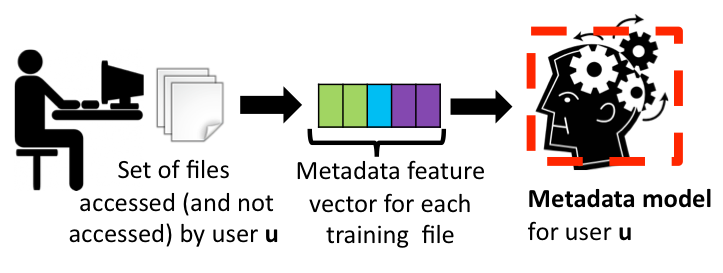
\includegraphics[trim = 0mm 0mm 0mm 4mm, clip, width=0.65\linewidth]{FileAccess/figs/meta_training} \\
\multicolumn{1}{l}{(a) \textbf{Training}: metadata models for each user} \\ 
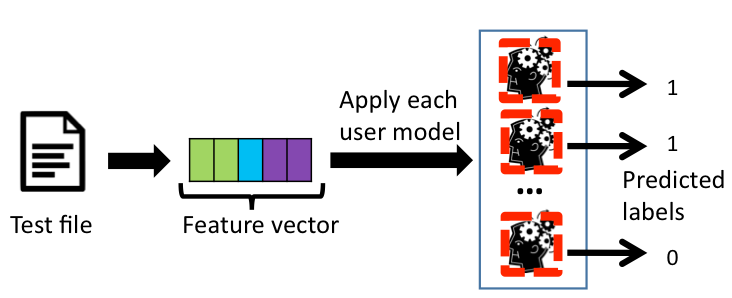
\includegraphics[trim = 0mm 0mm 0mm 7mm, clip, width=0.65\linewidth]{FileAccess/figs/testing} \\
\multicolumn{1}{l}{(b) \textbf{Testing}: apply the trained models for all users in share} \\  
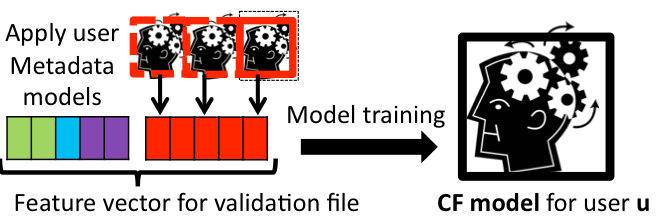
\includegraphics[width=0.62\linewidth]{FileAccess/figs/cf_training2} \\
\multicolumn{1}{l}{(c) \textbf{Training}: CF models for each user} \\  
\end{tabular}
}
\caption{Approach Overview}
\label{fig:overallfigs}
%\vspace{-0.5cm}
\end{figure}

%%
Our system uses a binary classification approach for providing file
recommendations.  For this purpose, it builds a separate
classification model for each user of a file share.  The dataset of a
given user includes all the files that have been accessed by all 
users of the share.  The label of a file in the dataset is $1$ if the
user accesses it, $0$ otherwise.  It is important to know that if a
user accesses a particular file during the training phase, it is
highly likely that the user will access the same file during the
testing phase.  Recommending such a file to the user is not very
useful.  Hence the main objective of our system is to discover useful
but new files that may have been created or modified by other users of
the same share.  For this reason, the testing phase includes only
those files that are new with respect to the training phase for the
user.  Our system then applies the model of the user to these files to
predict classification labels.  The rest of this section describes the
features and the modeling techniques used in the system.

%% The proposed system comprises of a training and a testing
%% phase. During training, file activities are monitored, features are
%% extracted from file metadata and a model per user is trained. This is shown
%% for metadata based models in Figure~\ref{fig:overallfigs}(a). During testing or classification phase (Figure~\ref{fig:overallfigs}(b)), features are
%% extracted from each created or modified file and the trained models for
%% every user in the share are applied on the file. The features used and modeling
%% techniques adopted are briefly described below.

%Details can be obtained from~\cite{dwiticeis15}. 
\subsection{Metadata Features}
\label{sec:features}
%%
The metadata features include features extracted from different
attributes of a file:
%% The metadata features of each training or test file are concatenation
%% of its folder, token and extension features.
%%
\begin{itemize}
  \renewcommand{\labelitemi}{$\bullet$}
%%
\item \textbf{Folder}:
%%
We create a folder feature corresponding to every folder and its
ancestor folders observed in the training period\footnote{Please note
  that no features are derived for completely new attributes seen only
  during the testing phase.}.  For a file $f$, we capture the folder
features as a binary vector with the value 1 in the locations
corresponding to the folder or the ancestor folders of $f$, and 0
elsewhere.  These features help in learning a user's preference for
certain subtrees of the file system hierarchy in a share without
having to define a folder distance metric.
%%
\item \textbf{Token}:
%%
We tokenize the path name of each file using a novel tokenization
approach, the details of which can be found in~\cite{dwiticeis15}.  We
construct a token vocabulary using all the tokens observed during the
training phase.  For extracting features, we capture tokens of a file
as bag-of-words representation on the entire vocabulary.
%%
\item \textbf{Extension}:
%%
We construct an extension vocabulary based on the popular extensions
observed in the training data.  We then use this vocabulary to
represent a file's extension with one-hot encoding-based features.
%%
\end{itemize}
%%
%% \begin{enumerate}
%% \item \textbf{Folder features}: We create a folder feature
%%   corresponding to every folder and its ancentor folders observed in
%%   the training period. For every training or test file $f$, its folder
%%   features are a binary vector with 1 in locations corresponding to
%%   the folder of $f$ or its ancenstors, and 0 elsewhere. This feature helps learning a user's
%% preferences for certain subtrees of the file system
%%   hierarchy in a share without the need of definining folder distance
%%   metrics.
%%
%% \item \textbf{Token features}: We tokenize the path name of each file using a novel tokenization approach, the details of which are given in ~\cite{dwiticeis15}. The tokens resulting observed during training are used to construct a token vocabulary. The tokens in each file's path are represented using bag of words representation on the constructed vocabulary. 

%% \item \textbf{Extension features}: We construct an extension vocabulary based on the popular extensions observed in the training data. One-hot encoding is
%%   used to represent the extension of each file based on the constructed extension vocabulary. 
%% \end{enumerate}
%The metadata features of a file are concatenation of its folder, token and extension features. 

\subsection{Modeling Techniques} 
\label{sec:Metamodels}
%%
We first build basic metadata models based on the metadata features.
Using these models, we then develop an innovative approach to leverage
collaboration among users for building collaborative filtering aware
models that provide better performance over the basic metadata models.
%% Our system trains per user models using the activity observed over a
%% training period. For user $u$, every file $f$ that has been read in
%% the training period is a training instance. The corresponding label is
%% 1 if $u$ has read $f$ during training, 0 otherwise. Thus while the
%% training instances for all users in a share are the same, the labels
%% may be different. For testing, every file that has been read in
%% testing period and has $not$ been seen in training is a testing
%% instance. Doing so ensures that the models are evaluated over files
%% that are new with respect to the training data. Testing labels are
%% determined in a similar manner as training labels. We approach file
%% recommendation as a classification problem and use the following
%% modeling approaches.
%Below are the two modeling aproaches used in our system. 

\subsubsection{Metadata-based Modeling}
%%
For each user, we train a metadata model using the metadata features.
Figure~\ref{fig:overallfigs} (a, b) shows the training and the testing
phases of this approach.  Considering the trade-off between accuracy
and training time efficiency~\cite{dwiticeis15}, we pick Support
Vector Machine (SVM) with a linear kernel as our modeling technique
because it provides high accuracy without incurring significant
training time.  More importantly, a linear SVM provides feature
weights that capture the relative significance of individual features.
We leverage this aspect in our scalability optimization technique AFMS
as described in Section~\ref{sec:testspeedup}.

%% For each user, we train a metadata based model using the metadata features of the training files and their labels. We have chosen Support Vector Machines (SVMs) with linear kernel as the models since they offer high accuracy without
%% incurring significant training time. \cite{dwiticeis15} provides a
%% comparison between different machine learning models. 
%% In addition, linear SVMs provide feature weights that can determine the significance of individual features, and can be leveraged for techniques such as Active Feature based Model Selection (Section~\ref{sec:testspeedup}) to improve the scalability of our system. 
%% The training and
%% testing for metadata based models is shown in
%% Figures~\ref{fig:overallfigs}(a) and \ref{fig:overallfigs}(b)
%% respectively.
\subsubsection{Collaborative Filtering (CF)-based Modeling} 
\label{sec:CFdetails}
%%
Enterprise users often show a high degree of collaboration in terms of
accessing common files in a share.  We make this observation based on
the measurement of the metric, \textit{normalized triangle count} 
(Section~\ref{sec:data}), that captures the degree of collaboration
among users.  As an illustration, see Figure~\ref{fig:snagraphs} that
shows user communities in terms of social network graphs for a couple
of shares.

We leverage user collaborations to build CF models that are
significantly more effective than the metadata models.  Here are the
details of the method used in building a CF model for a user $u$.
First, we divide the original training set into a new training set and a
validation set.  We then use the new training set to train a metadata
model for each user.  Second, for each file in the validation set, we
apply the metadata models of all the users, and generate a vector of
the resulting predicted labels.  Third, we train the CF model for the
user $u$ using the files in the validation set.  For this, we
construct the feature vector for each validation file by concatenating
the metadata features with the vector of the predicted labels
(Figure~\ref{fig:overallfigs}(c)).  For each test file observed during
the testing phase, we first apply the metadata models of all the users
to generate a vector of the predicted labels.  Finally, we append this
vector to the metadata features to create a new feature vector and
feed it to the user $u$'s CF model to obtain the final predicted
label.


An interesting point to be noted here is that our CF-based modeling
technique does not require a pre-defined user-user relationship or
even a user similarity metric.  Rather, the model can automatically learn
positive or negative correlation between the activities of users, and
accordingly adapt to make better predictions.  For instance, if two
users have similar access patterns, the CF model for one user could
learn that its labels positively correlate with labels predicted by
the other user's metadata model.  Thus, greater the degree of
collaboration, the better will be the effectiveness of the CF models.
Another benefit of our technique is that, unlike pure collaborative
filtering-based systems developed in the past, it does not suffer from
a cold-start problem.  Previous systems recommend an item to a user if
other \textit{similar} users have shown a preference for that item.
Therefore, these systems are incapable of recommending a completely
new item because no other user has seen it before.  In contrast, the
novelty of our technique is in using CF features that are based on
predicted labels rather than the history of past accesses.

%% Enterprise users demonstrate a high degree of collaboration in terms
%% of accessing common files in a share. This is validated in Section~\ref{sec:data} where we measure the collaboration among users in terms of normalized triangle counts and also demonstrate the existence of user communities in social network graphs for sample shares. For each user, we train a CF aware model that captures the
%% predictions of all metadata based user models in a share with the aim of making
%% better prediction for the user by leveraging user
%% collaboration. In order to do this, we divide the set of training files into training and validation files. The metadata based models corresponding to each user in a share are trained on the training files and each
%% metadata model is applied on each validation files, resulting
%% in a vector of predicted metadata model based labels per validation file. 
%% The CF aware model for each user is then trained using all validation files. The features used for each validation file are concatenation of its metadata features, and the vector of predicted metadata model based labels for the file. This is shown in
%% Figure~\ref{fig:overallfigs}(c). On a test file, first the metadata
%% based models of all users in a share are applied to obtain the
%% predicted metadata model based labels. They are then concatenated with the file's metadata
%% features and the CF aware models are then applied to obtain the final predicted label for the user.
%% %Such an approach enables capturing the relationships between predictions of different users in a share. 

%% The CF aware modeling as proposed above does not require a pre-defined user-user relationship or even a similarity metric. Rather, the model can automatically learn if there is positive or negative correlation between the activities of users, and accordingly adapt the model to use this information to make better predictions. For example if two users have similar access patterns, then the CF aware model for one user could learn that its labels typically correlate with labels predicted by the other user's metadata based model. It is expected that CF aware models can provide most benefit in a share that demonstrates substantial user collaboration. 
%% Another benefit of using the above approach is that unlike purely collaborative filtering based systems, the proposed approach does not suffer from cold-start problem. Systems that recommend items to a user if other \textit{similar} users have liked, accessed or purchased the item are incapable of recommending items that are completely new since there are no users who have already accessed it. As compared to these, the collaboration based features that are utilized in the CF aware models are based on \textit{predicted} labels instead of actual past accesses and are used in addition to metadata features. 

